%Om filen typsätts som del av hela rapporten så finns \master definierat i början och ingen \begin{document} och \end{document} får finnas, men för att kunna typsätta filen för sig är dem ett måste! \newcommand{\master}{} krävs i början på huvudrapporten!
\ifdefined\master
\else
	\documentclass[twocolumn]{article}
	\usepackage{graphicx}
	\usepackage{float}
	%\input{../preamble}
	\begin{document}
\fi

\subsection{Inputs}
Lab Assistant supports two types of devices for input; function generators and voltage generators. The function generator can also be used to generate a frequency sweep.

\subsubsection*{Function Generator}
Uses function generator to output a signal. The \emph{waveform} popup-menu sets the signal type to sine, square, triangle or sawtooth. If no waveform is selected the current waveform of the function generator is used. \emph{Frequency}, \emph{amplitude} and \emph{offset} controlls the parameters of the output. In order to establish a connection to the function generator its GPIB-address must be put into the \emph{GPIB-address} field. (Figure \ref{fig:funcgen})

\begin{figure}[H]
\centering
\fbox{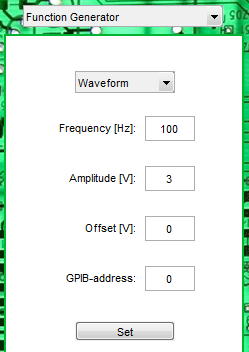
\includegraphics[width=4cm]{Figure/function_generator.png}}
\caption{Function Generator settings.}
\label{fig:funcgen}
\end{figure}

\subsubsection*{Frequency Sweep}
The function generator can also be used to generate a Bode plot of a connected system. When \emph{frequency sweep} is selected as input, output is automatically set to \emph{bode graph} and no other outputs can be chosen. Available settings for the sweep are \emph{start frequency}, \emph{end frequency}, \emph{step length} and \emph{amplitude}. GPIB-address must allso be filled in as described above.  (Figure \ref{fig:freqsw})

\begin{figure}[H]
\centering
\fbox{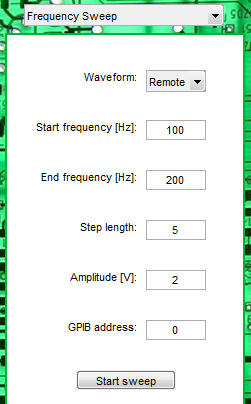
\includegraphics[width=4cm]{Figure/frequency_sweep.png}}
\caption{Frequency sweep settings.}
\label{fig:freqsw}
\end{figure}

\subsubsection*{Voltage Generator}
The other device supported is the voltage generator. Apart from \emph{GPIB-Address} of the voltage generator, the available settings are \emph{voltage} and \emph{current limit}. Output can be toggled with the \emph{output on/off} pushbutton. (Figure \ref{fig:voltgen})

\begin{figure}[H]
\centering
\fbox{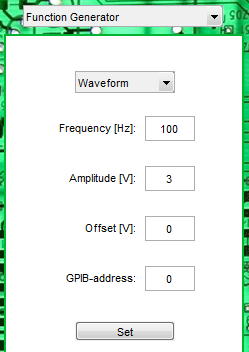
\includegraphics[width=4cm]{Figure/function_generator.png}}
\caption{Voltage Generator settings.}
\label{fig:voltgen}
\end{figure}

\ifdefined\master
\else
	\end{document}
\fi